\label{sec:geom}

The \verb+GEOMETRY+ directive is a compound directive that allows the
user to define the geometry to be used for a given calculation.  The
directive allows the user to specify the geometry with a relatively
small amount of input, but there are a large number of optional
keywords and additional subordinate directives that the user can
specify, if needed.  The directive therefore appears to be rather long
and complicated when presented in its general form, as follows:
\begin{verbatim}
  GEOMETRY [<string name default geometry>] \
           [units <string units default angstroms>] \
           [(angstrom_to_au || ang2au) \
                  <real angstrom_to_au default 1.8897265>] \
           [print [xyz] || noprint] \
           [center || nocenter] \
           [bqbq] \
           [autosym [real tol default 1d-2]] \
           [autoz || noautoz] \
           [adjust] \
           [(nuc || nucl || nucleus) <string nucmodel>]
           
    
    [SYMMETRY [group] <string group_name> [print] \
           [tol <real tol default 1d-2>]]



    <string tag> <real x y z> [vx vy vz] [charge <real charge>] \
           [mass <real mass>] \
           [(nuc || nucl || nucleus) <string nucmodel>]
    ... ]

    [ZMATRIX || ZMT || ZMAT
         <string tagn> <list_of_zmatrix_variables>
         ... 

         [VARIABLES
              <string symbol> <real value>
              ... ]
 
         [CONSTANTS
              <string symbol> <real value>
              ... ]

     (END || ZEND)]

         [ZCOORD
              CVR_SCALING <real value>
              BOND    <integer i> <integer j> \
                      [<real value>] [<string name>] [constant]
              ANGLE   <integer i> <integer j> \
                      [<real value>] [<string name>] [constant]
              TORSION <integer i> <integer j> <integer k> <integer l> \
                      [<real value>] [<string name>] [constant]
          END]
          
          [SYSTEM surface  <molecule polymer surface crystal default molecule>
               lat_a <real lat_a> lat_b <real lat_b> lat_c <real lat_c>
               alpha <real alpha> beta <real beta> gamma <real gamma>
          END]
 
   END


\end{verbatim}

The three main parts of the \verb+GEOMETRY+ directive
are:

\begin{itemize}
\item keywords on the first line of the directive (to specify such optional
input as the geometry name, input units, and print level for the output)
\item symmetry information
\item Cartesian coordinates or Z-matrix input to specify the locations 
of the atoms and centers
\item lattice parameters (needed only for periodic systems)
\end{itemize}

The following sections present the input for this compound directive in
detail, describing the options available and the usages of the various
keywords in each of the three main parts.


\section{Keywords on the {\tt GEOMETRY} directive}
\label{sec:geomkeys}

This section presents the options that can be specified using the keywords 
and optional input on the main line of the {\tt GEOMETRY} directive.
As described above, the first line of the directive has the general form,
\begin{verbatim}
  GEOMETRY [<string name default geometry>] \
           [units <string units default angstroms>] \
           [bqbq] \
           [print [xyz] || noprint] \
           [center || nocenter] \
           [autosym [real tol default 1d-2]] \
           [autoz || noautoz] \
           [adjust] \
           [(nuc || nucl || nucleus) <string nucmodel>]
\end{verbatim}
    
All of the keywords and input on this line are optional.  The following
list describes  all options and their defaults.

\begin{itemize}
\item \verb+<name>+ -- user-supplied name for the geometry; the
  default name is \verb+geometry+, and all NWChem modules look for a
  geometry with this name.  However, multiple geometries may
  be specified by using a different name for each.  Subsequently,
  the user can direct a module to a named geometry by
  using the \verb+SET+ directive (see
  the example in Section \ref{sec:set}) to associate the default
  name of \verb+geometry+ with the alternate name.

% \subsection*{{\tt UNITS}}
\item \verb+units+ -- keyword specifying that a value will be entered
  by the user for the string variable \verb+<units>+.  The default
  units for the geometry input are \angstroms\ (Note: atomic units or
  Bohr are used within the code, regardless of the option specified
  for the input units.  The default conversion factor used in the code
  to convert from {\angstroms} to Bohr is $1.8897265$ which may be
  overidden with the \verb+angstrom_to_au+ keyword described below.).  The code
  recognizes the following possible values for the string variable
  \verb+<units>+:
\begin{itemize}
\item \verb+angstroms+ or \verb+an+ --- Angstroms (\AA), the default
  (converts to A.U. using the \AA to A.U. conversion factor)
\item \verb+au+ or \verb+atomic+ or \verb+bohr+ --- Atomic units (A.U.)
\item \verb+nm+ or \verb+nanometers+ --- nanometers (converts to
  A.U. using a conversion factor computed as $10.0$ times the
  \AA\ to A.U. conversion factor) 
\item \verb+pm+ or \verb+picometers+ --- picometers (converts to 
  A.U. using a conversion factor computed as $0.01$ times the 
  \AA\ to A.U. conversion factor)
\end{itemize}

\item \verb+angstrom_to_au+ -- may also be specified as
  \verb+ang2au+.  This enables the user to modify the conversion
  factors used to convert between \AA\ and A.U..  The default value is
  $1.8897265$. 
      
\item \verb+bqbq+ -- keyword to specify the treatment of interactions
  between dummy centers.  The default in NWChem is to ignore such
  interactions when computing energies or energy derivatives.  These
  interactions will be included if the keyword \verb+bqbq+ is
  specified.

\item \verb+print+ and \verb+noprint+ -- complementary keyword pair to
  enable or disable printing of the geometry.  The default is to print
  the output associated with the geometry.  In addition, the keyword
  \verb+print+ may be qualified by the additional keyword \verb+xyz+,
  which specifies that the coordinates should be printed in the XYZ
  format of molecular graphics program XMol.

\item \verb+center+ and \verb+nocenter+ -- complementary keyword pair
  to enable or disable translation of the center of nuclear charge to
  the origin.  With the origin at this position, all three components
  of the nuclear dipole are zero.  The default is to move the center
  of nuclear charge to the origin.

\item \verb+autosym+ -- keyword to specify that the symmetry of the
  geometric system should be automatically determined.  This option is on
  by default.  Only groups up to and including $O_{h}$ are recognized.
  Occasionally NWChem will be unable to determine the full symmetry
  of a molecular system, but will find a proper subgroup of the full 
  symmetry.  The default tolerance is set to work for most cases, but may
  need to be decreased to find the full symmetry of a geometry.  Note that
  autosym will be turned off if the \verb+SYMMETRY+ group input is given
  (See section \ref{sec:symgrp}).

\item \verb+noautoz+ -- by default NWChem (release 3.3 and later) 
  will generate redundant internal coordinates from user input
  Cartesian coordinates.  The internal coordinates will be used in
  geometry optimizations.  The \verb+noautoz+ keyword disables use of
  internal coordinates.  The \verb+autoz+ keyword is provided only for
  backward compatibility.  See Section \ref{sec:zcoord} for a more
  detailed description of redundant internal coordinates, including
  how to force the definition of specific internal variables in
  combination with automatically generated variables.

\item \verb+adjust+ -- This indicates that an existing geometry is
  to be adjusted.  Only new input for the redundant internal
  coordinates may be provided (Section \ref{sec:zcoord}).  It is 
  not possible to define new centers or to modify the point
  group using this keyword.  See Section \ref{sec:zcoord} for 
  an example of its usage.

\item \verb+nucleus+ -- keyword to specify the default model for the nuclear
  charge distribution. The following values are recognized:
\begin{itemize}
\item \verb+point+ or \verb+pt+ --- point nuclear charge distribution. This
  is the default.
\item \verb+finite+ or \verb+fi+ --- finite nuclear charge distribution
  with a Gaussian shape. The RMS radius of the Gaussian is determined from
  the nuclear mass number $A$ by the expression 
  $r_{\rm RMS} = 0.836*A^{1/3}+0.57$ fm.
\end{itemize}
NOTE: If you specify a finite nuclear size, you should ensure that the basis
set you use is contracted for a finite nuclear size.  See the Section
\ref{sec:basis} for more information.

\end{itemize}

The following examples illustrate some of the various options that the
user can specify on the first input line of the \verb+GEOMETRY+
directive, using the keywords and input options described above.

The following directives all specify the same geometry for $H_2$ (a
bond length of 0.732556\ \AA):
\begin{verbatim}
  geometry                           geometry units nm    
    h 0 0 0                            h 0 0 0            
    h 0 0 0.732556                     h 0 0 0.0732556    
  end                                end                  

  geometry units pm                  geometry units atomic 
    h 0 0 0                            h 0 0 0             
    h 0 0 73.2556                      h 0 0 1.3843305     
  end                                end                   
\end{verbatim}
      
\section{{\tt SYMMETRY} --- Symmetry Group Input}
\label{sec:symgrp}

The \verb+SYMMETRY+ directive is used (optionally) within the compound
\verb+GEOMETRY+ directive to specify the point group for the molecular
geometry. 
The general form of the directive, as described above within the general
form of the \verb+GEOMETRY+ directive, is as follows:
\begin{verbatim}
    [SYMMETRY [group] <string group_name> [print] \
           [tol <real tol default 1d-2>]]
\end{verbatim}
The keyword \verb+group+ is optional, and can be omitted without
affecting how the input for this directive is processed\footnote{For
  periodic systems, there are additional keywords within this
  directive (not yet documented), so having a keyword for the group
  name is useful.}.  However, if the \verb+SYMMETRY+ directive is
used, a group name must be specified by supplying an entry for the
string variable \verb+<group_name>+.  The group name should be
specified as the standard Sch\"{o}flies symbol.  Examples of expected
input for the variable \verb+group_name+ include such entries as:

\begin{itemize}
\item \verb+c2v+ -- for molecular symmetry $C_{2{\it v}}$
\item \verb+d2h+ -- for molecular symmetry $D_{2h}$
\item \verb+Td+ -- for molecular symmetry $T_d$
\item \verb+d6h+ -- for molecular symmetry $D_{6h}$
\end{itemize}

The \verb+SYMMETRY+ directive is optional.  The default is no symmetry 
(i.e., $C_1$ point group). Automatic detection of point
group symmetry is available through the use of \verb+autosym+ in the
\verb+GEOMETRY+ directive main line (discussed in Section \ref{sec:geomkeys}).
Note: if the \verb+SYMMETRY+ directive is present the \verb+autosym+
keyword is ignored.

If only symmetry-unique atoms are specified, the others will be
generated through the action of the point group operators, but the
user if free to specify all atoms.  The user must know the symmetry of
the molecule being modeled, and be able to specify the coordinates of
the atoms in a suitable orientation relative to the rotation axes and
planes of symmetry.  Appendix \ref{symexamples} lists a number of
examples of the
\verb+GEOMETRY+ directive input for specific molecules having symmetry
patterns recognized by NWChem.  The exact point group symmetry will be
forced upon the molecule, and atoms within $10^{-3}$ A.U. of a
symmetry element (e.g., a mirror plane or rotation axis) will be
forced onto that element.  Thus, it is not necessary to specify to a
high precision those coordinates that are determined solely by
symmetry.

The keyword \verb+print+ gives information concerning the point group
generation, including the group generators, a character table, the
mapping of centers, and the group operations.

The keyword \verb+tol+ relates to the accuracy with which the symmetry-unique
atoms should be specified.  When the atoms are generated, those that are
within the tolerance, \verb+tol+, are considered the same.

\section{Cartesian coordinate input}
\label{sec:cart}

The default in NWChem is to specify the geometry information entirely
in Cartesian coordinates, and examples of this format have 
appeared above (e.g, Section \ref{sec:realsample}). Each center
(usually an atom) is identified on a line of the following form:
\begin{verbatim}

    <string tag> <real x y z> [vx vy vz] \
        [charge <real charge>] [mass <real mass>] \
        [(nuc || nucl || nucleus) <string nucmodel>]

\end{verbatim}

The string \verb+<tag>+ is the name of the atom or center, and its case
(upper or lower) is important.  The tag is limited to 16 characters
and is interpreted as follows:
\begin{itemize}
\item If the entry for \verb+<tag>+ begins with either the symbol or
  name of an element (regardless of case), then the center is treated
  as an atom of that type.  The default charge is the atomic number
  (adjusted for the presence of ECPs by the ECP \verb+NELEC+ directive
  ; see Section \ref{sec:ecp}).  Additional characters can be added to
  the string, to distinguish between atoms of the same element (For
  example, the tags \verb+oxygen+, \verb+O+, \verb+o34+,
  \verb+olonepair+, and \verb+Oxygen-ether+, will all be interpreted
  as oxygen atoms.).
\item If the entry for \verb+<tag>+ begins with the characters
  \verb+bq+ or \verb+x+ (regardless of case), then the center is
  treated as a dummy center with a default zero charge (Note: a tag
  beginning with the characters \verb+xe+ will be interpreted as a
  xenon atom rather than as a dummy center.).  Dummy centers may
  optionally have basis functions or non-zero charge.  See Section
  \ref{sec:sample2} for a sample input using dummy centers with
  charges.
\end{itemize}

It is {\em important} to be aware of the following points regarding
the definitions and usage of the values specified for the variable
\verb+<tag>+ to describe the centers in a system:
\begin{itemize}
\item If the tag begins with characters that cannot be matched against
  an atom, and those characters are not \verb+BQ+ or \verb+X+, then a
  fatal error is generated.
\item The tag of a center is used in the \verb+BASIS+ (Section
  \ref{sec:basis}) and \verb+ECP+ (Section \ref{sec:ecp}) directives
  to associate functions with centers.
\item All centers with the same tag will have the same basis
  functions.
\item When using automatic symmetry detection,
  only centers with the same tag will be candidates for testing for
  symmetry equivalence.
\item The user-specified charges (of all centers, atomic and dummy)
  and any net total charge of the system (Section \ref{sec:charge})
  are used to determine the number of electrons in the system.
\end{itemize}

The Cartesian coordinates of the atom in the molecule are specified as
real numbers supplied for the variables \verb+x+, \verb+y+, and
\verb+z+ following the characters entered for the tag.  The values
supplied for the coordinates must be in the units specified by the
value of the variable \verb+<units>+ on the first line of the
\verb+GEOMETRY+ directive input.

After the Cartesian coordinate input, optional velocities may be 
entered as real numbers for the variables \verb+vx+, \verb+vy+, and 
\verb+vz+.  The velocities should be given in atomic units and are 
used in QMD and PSPW calculations.

The Cartesian coordinate input line also contains the optional keywords
\verb+charge+, \verb+mass+ and \verb+nucleus+, which allow the user to
specify the charge of the atom (or center) and its mass (in atomic mass
units), and the nuclear model.  The default charge for an atom is
its atomic number, adjusted for the presence of ECPs (see Section
\ref{sec:ecp}).  In order to specify a different value for the charge on a
particular atom, the user must enter the keyword \verb+charge+, followed by
the desired value for the variable \verb+<charge>+.

The default mass for an atom is taken to be the mass of its most abundant
naturally occurring isotope or of the isotope with the longest half-life.
To model some other isotope of the element, its mass must be defined
explicitly by specifying the keyword \verb+mass+, followed by the value (in
atomic mass units) for the variable \verb+<mass>+.

The default nuclear model is a point nucleus. The keyword \verb+nucleus+ (or
\verb+nucl+ or \verb+nuc+) followed by the model name \verb+<nucmodel>+ 
overrides this default. Allowed values of \verb+<nucmodel>+ are \verb+point+ or
\verb+pt+ and \verb+finite+ or \verb+fi+. The \verb+finite+ option is
a nuclear model with a Gaussian shape. The RMS radius of the Gaussian is
determined by the atomic mass number via the formula $r_{\rm RMS} = 0.836*
A^{1/3} + 0.57$ fm.  The mass number $A$ is derived from the variable
\verb+<mass>+.

The geometry of the system can be specified entirely in Cartesian
coordinates by supplying a \verb+<tag>+ line of the type described
above for each atom or center.  The user has the option, however, of
supplying the geometry of some or all of the atoms or centers using a
Z-matrix description.  In such a case, the user supplies the input tag
line described above for any centers to be described by Cartesian
coordinates, and then specifies the remainder of the system using the
optional \verb+ZMATRIX+ directive described below in Section
\ref{sec:Z-matrix}.

\section{{\tt ZMATRIX} --- Z-matrix input}
\label{sec:Z-matrix}

The \verb+ZMATRIX+ directive is an optional directive that can be used
within the compound \verb+GEOMETRY+ directive to specify the structure
of the system with a Z-matrix, which can include both internal and
Cartesian coordinates.  The \verb+ZMATRIX+ directive is itself a
compound directive that can include the \verb+VARIABLES+ and
\verb+CONSTANTS+ directives, depending on the options selected.  The
general form of the compound \verb+ZMATRIX+ directive is as follows:
\begin{verbatim}
    [ZMATRIX || ZMT || ZMAT
         <string tagn> <list_of_zmatrix_variables> 
         ... 

         [VARIABLES
              <string symbol> <real value>
              ... ]
 
         [CONSTANTS
              <string symbol> <real value>
              ... ]

    (END || ZEND)]
\end{verbatim}

The input module recognizes three possible spellings of this directive
name.  It can be invoked with \verb+ZMATRIX+, \verb+ZMT+, or
\verb+ZMAT+.  The user can specify the molecular structure using
either Cartesian coordinates or
internal coordinates (bond lengths, bond angles and dihedral angles.
The Z-matrix input for a center defines connectivity, bond length, and
bond or torsion angles.  Cartesian coordinate input for a center
consists of three real numbers defining the x,y,z coordinates of the
atom.

Within the Z-matrix input, bond lengths and Cartesian coordinates must
be input in the user-specified units, as defined by the value specified
for the variable \verb+<units>+ on the first line of the \verb+GEOMETRY+
directive.  All angles are specified in
degrees.

The individual centers (denoted as \verb+i+, \verb+j+, and \verb+k+
below) used to specify Z-matrix connectivity may be designated either
as integers (identifying each center by number) or as tags ({\em If
  tags are used, the tag must be unique for each center.}) The use of
``dummy'' atoms is possible, by using \verb+X+ or \verb+BQ+ at the
start of the tag.

Bond lengths, bond angles and dihedral angles (denoted below as {\tt
  R}, {\tt alpha}, and {\tt beta}, respectively) may be specified
either as numerical values or as symbolic strings that must be
subsequently defined using the \verb+VARIABLES+ or \verb+CONSTANTS+
directives. The numerical values of the symbolic strings labeled
\verb+VARIABLES+ may be subject to changes during a geometry
optimization say, while the numerical values of the symbolic strings
labeled \verb+CONSTANTS+ will stay frozen to the value given in the
input.  The same symbolic string can be used more than once, and
any mixture of numeric data and symbols is acceptable. Bond angles
($\alpha$) must be in the range $0 < \alpha < 180$.

The Z-matrix input is specified sequentially as follows:
\begin{verbatim}
   tag1
   tag2 i R
   tag3 i R j alpha
   tag4 i R j alpha k beta [orient]
   ...
\end{verbatim}

The structure of this input is described in more detail below.  In the
following discussion, the tag or number of the center being currently
defined is labeled as \verb+C+ (``C'' for current).  The values
entered for these tags for centers defined in the Z-matrix input are
interpreted in the same way as the \verb+<tag>+ entries for Cartesian
coordinates described above (see Section \ref{sec:cart}).  Figures
\ref{fig:zmat1}, \ref{fig:zmat2} and \ref{fig:zmat3} display the
relationships between the input data and the definitions of centers
and angles.

\begin{figure}[htbp]
\centering
\begin{latexonly}
\ifx\pdfoutput\undefined
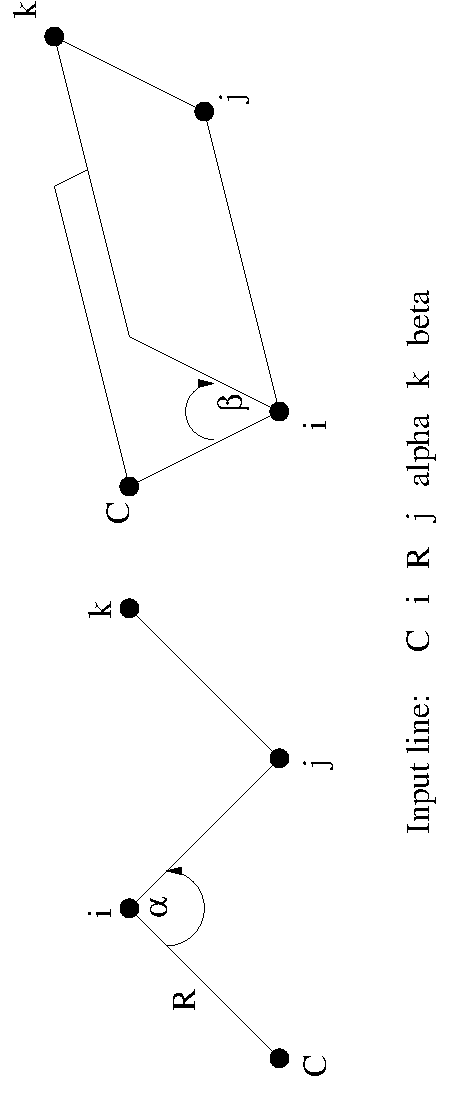
\includegraphics[angle=270,width=6in]{zmat1.eps}
\else
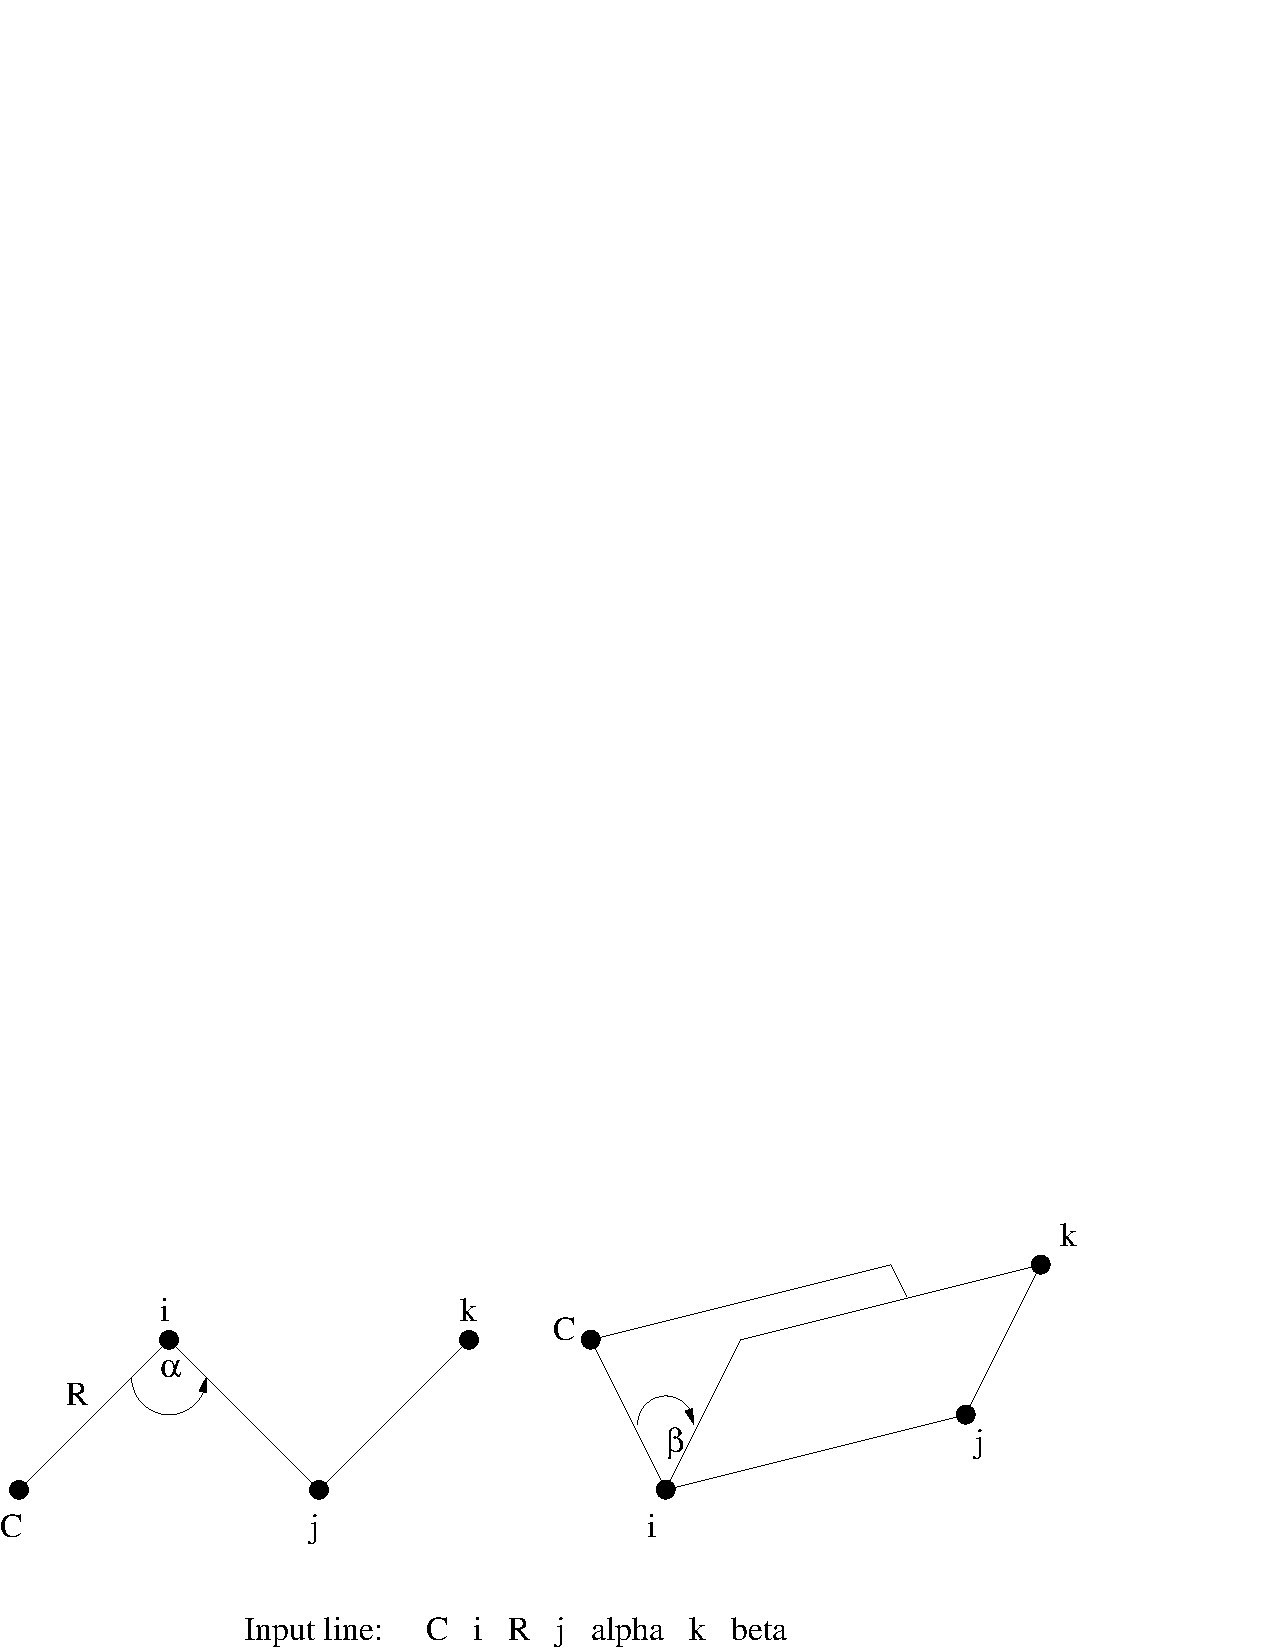
\includegraphics[angle=0,width=6in]{zmat1.pdf}
\fi
\end{latexonly}
\begin{htmlonly}
\psfig{figure=zmat1.eps,angle=270,width=6in}
\end{htmlonly}
\caption{\label{fig:zmat1} Relationships between the centers, bond angle
and dihedral angle in Z-matrix input.}
\end{figure}

\begin{figure}[htbp]
\centering
\begin{latexonly}
\ifx\pdfoutput\undefined
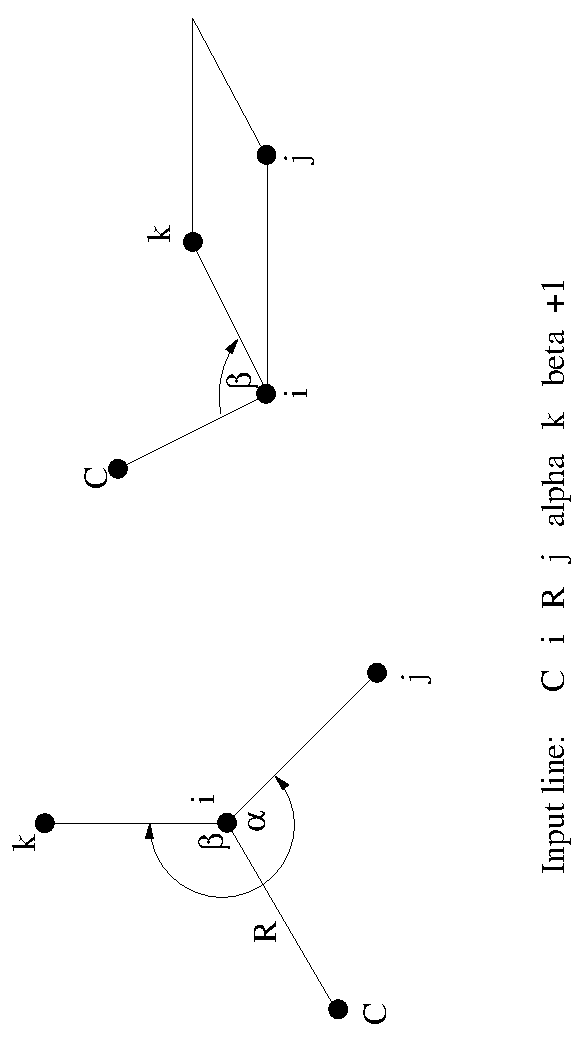
\includegraphics[angle=270,width=6in]{zmat2.eps}
\else
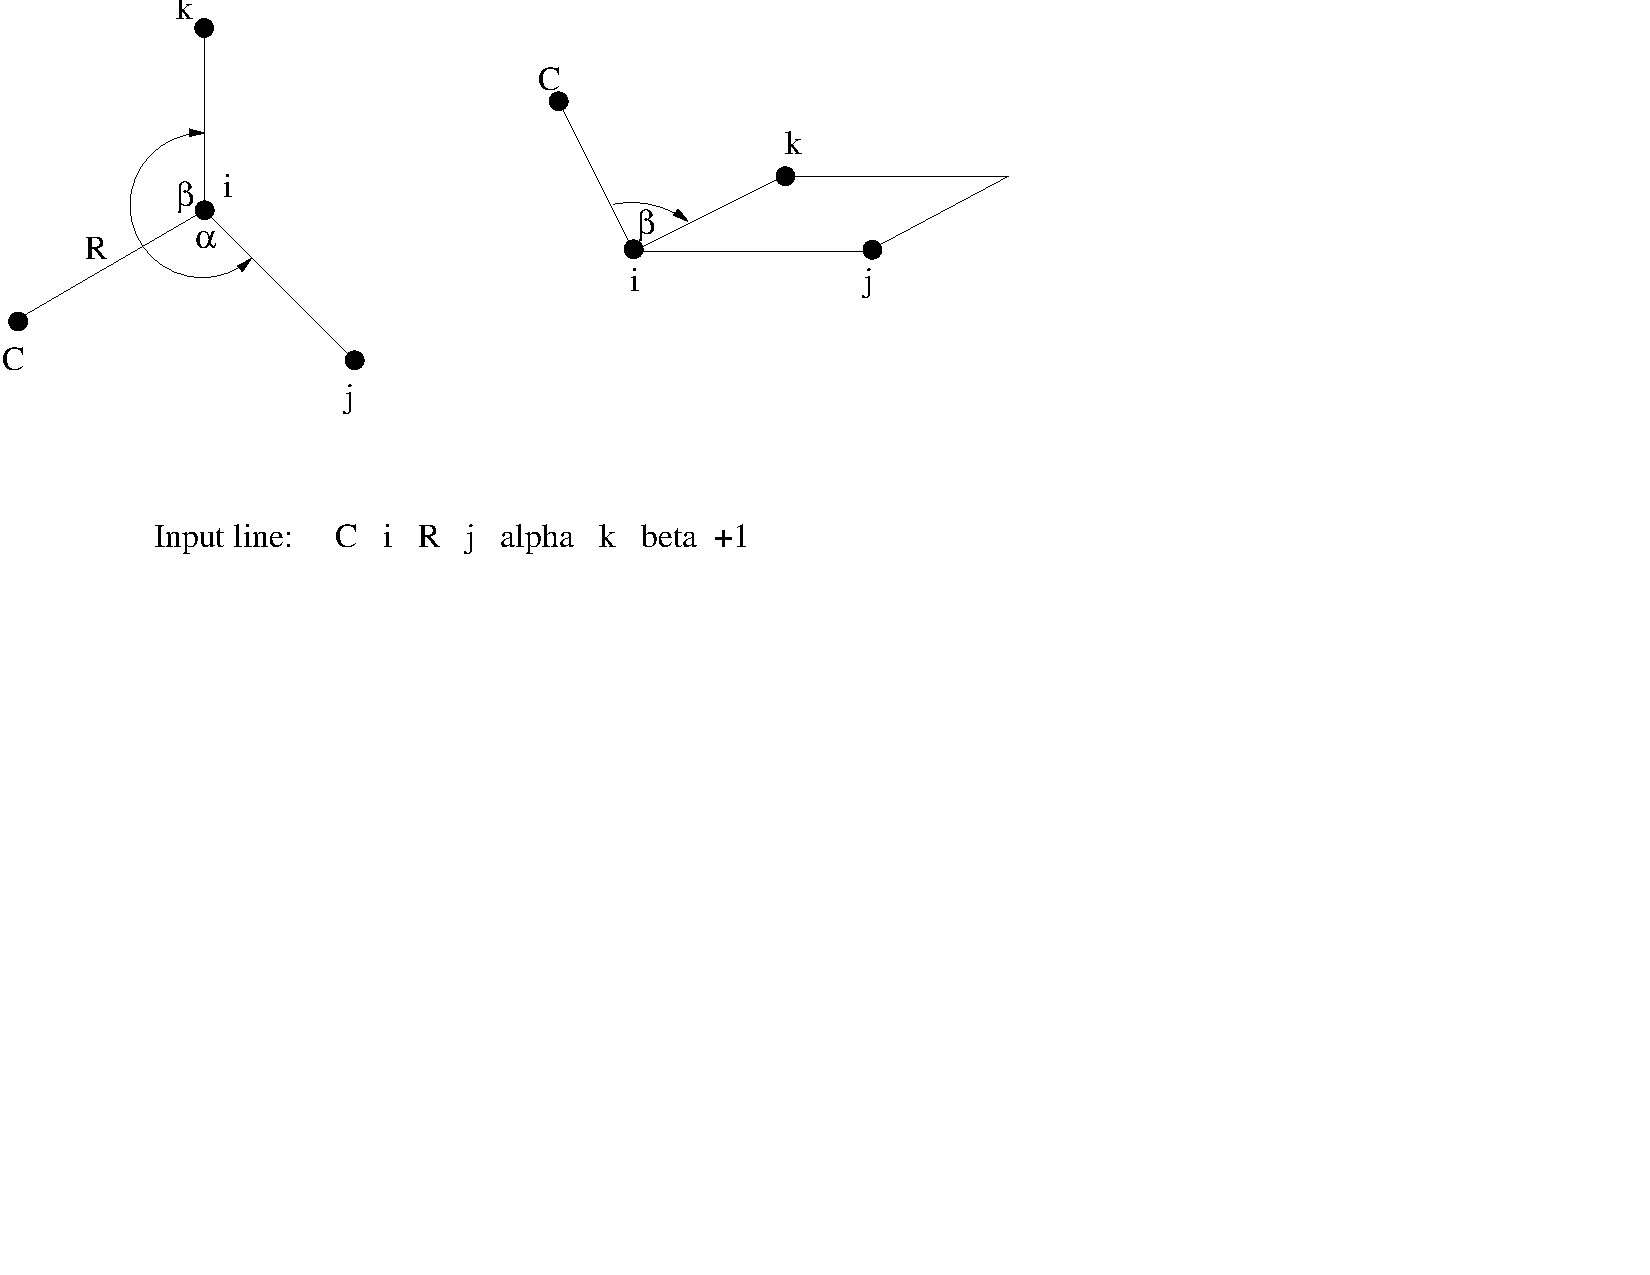
\includegraphics[angle=270,width=6in]{zmat2.pdf}
\fi
\end{latexonly}
\begin{htmlonly}
\psfig{figure=zmat2.eps,angle=270,width=6in}
\end{htmlonly}

\caption{\label{fig:zmat2} Relationships between the centers and two
  bond angles in Z-matrix input with optional parameter specified as $+1$.}
\end{figure}

\begin{figure}[htbp]
\centering
\begin{latexonly}
\ifx\pdfoutput\undefined
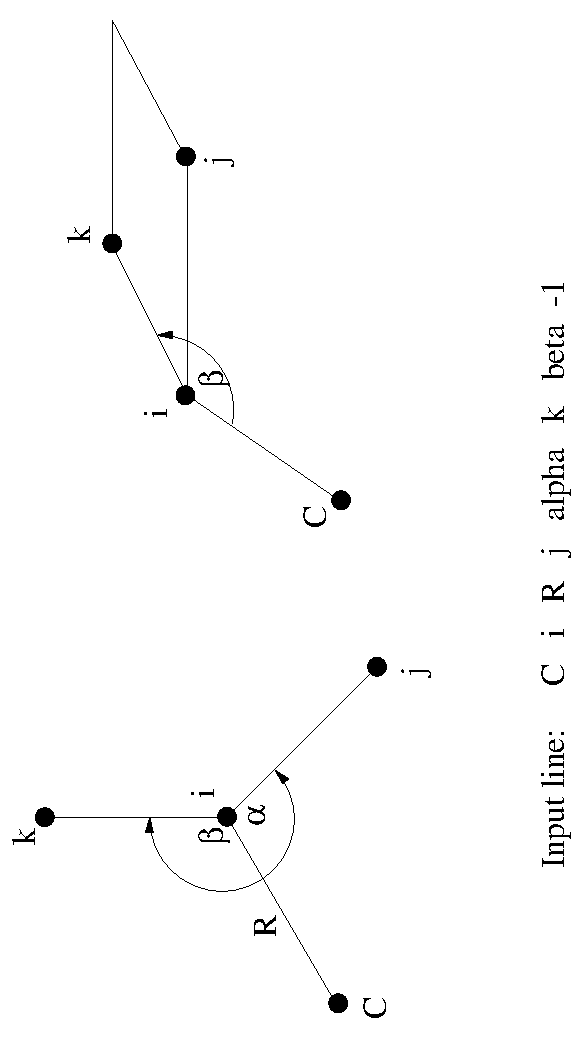
\includegraphics[angle=270,width=6in]{zmat3.eps}
\else
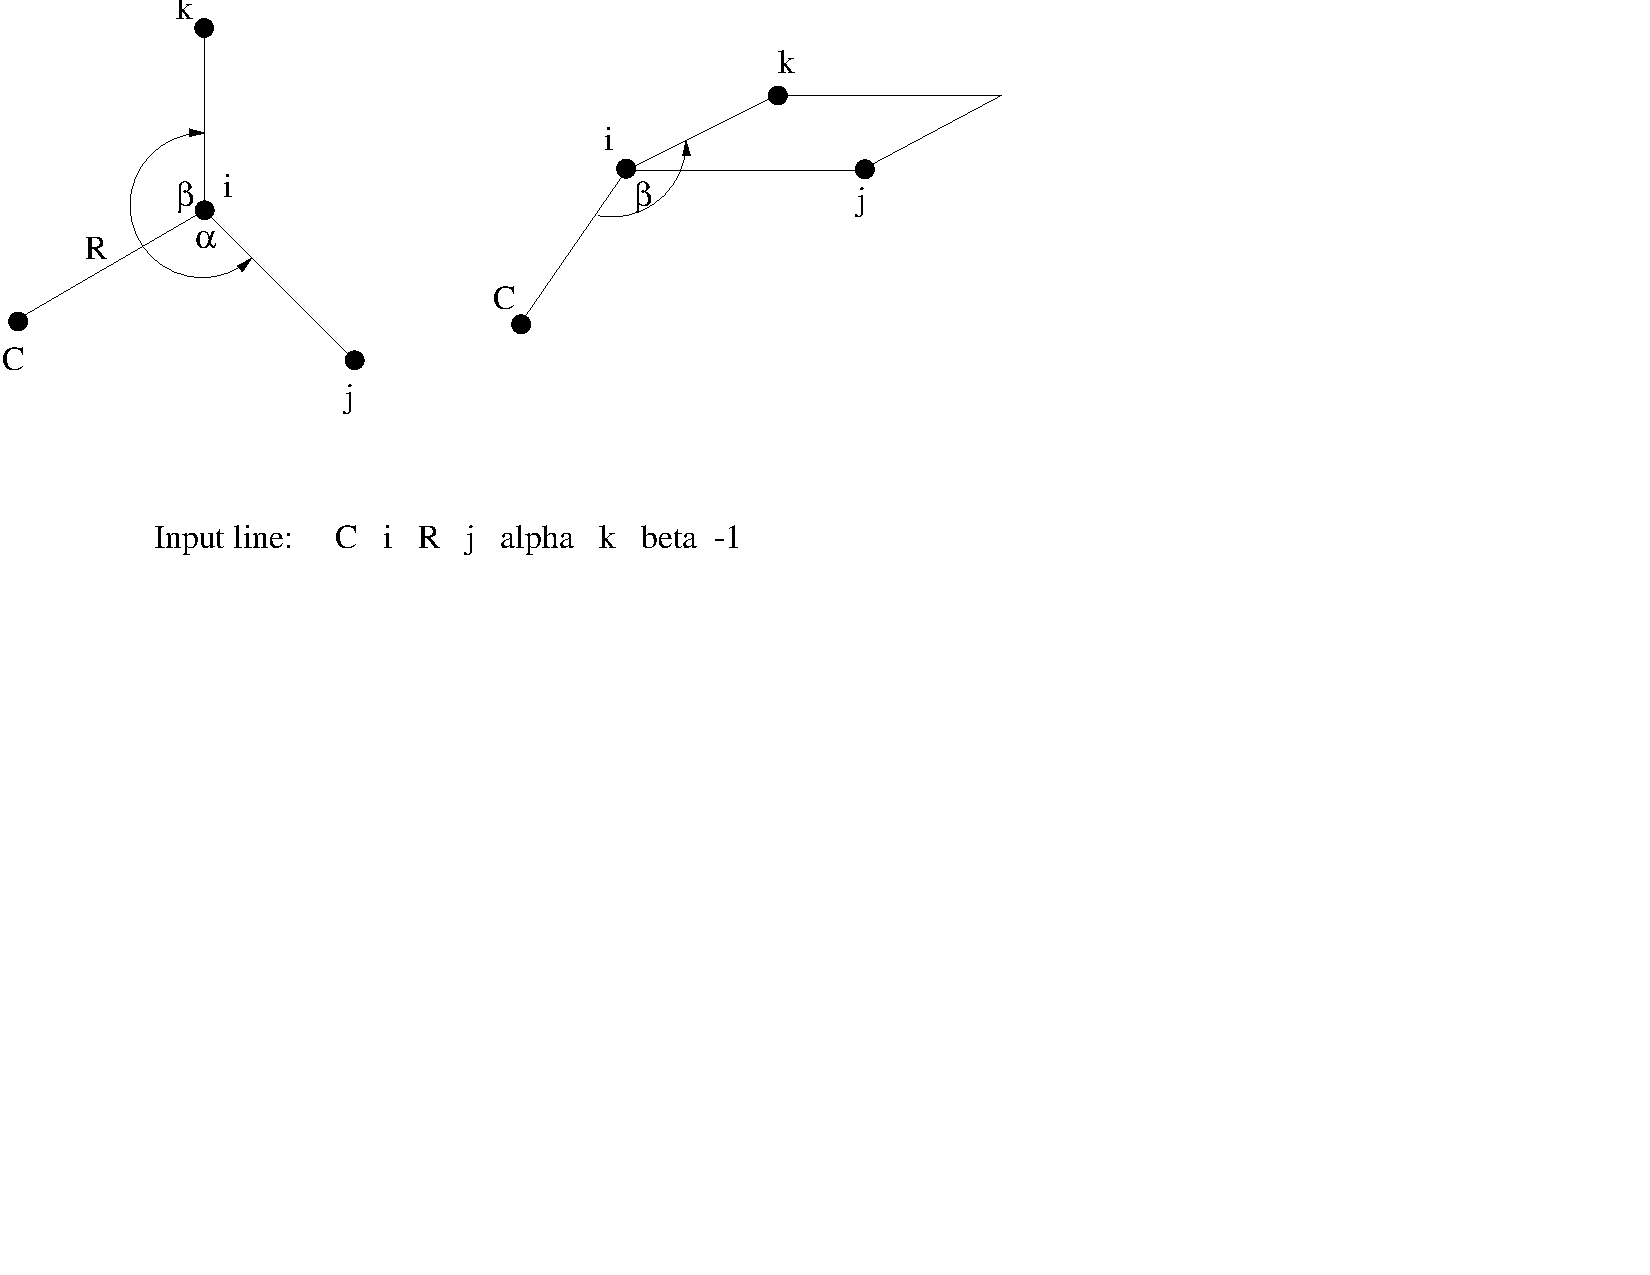
\includegraphics[angle=270,width=6in]{zmat3.pdf}
\fi
\end{latexonly}
\begin{htmlonly}
\psfig{figure=zmat3.eps,angle=270,width=6in}
\end{htmlonly}
\caption{\label{fig:zmat3} Relationships between the centers and two
  bond angles in Z-matrix input with optional parameter specified as $-1$.}
\end{figure}

The Z-matrix input shown above is interpreted as follows:
\begin{enumerate}

   \item \verb+tag1+

   Only  a  tag  is required for the first center.

   \item \verb+tag2 i R+

     The second center requires specification of its tag and the
     bond length ($R_{Ci}$) distance to a previous atom, which is identified by
     \verb+i+.

   \item \verb+tag3 i R j alpha+

     The third center requires specification of its tag, its bond length distance
     ($R_{Ci}$) to one of the two previous centers (identified by the
     value of \verb+i+), and the bond angle $\alpha = \widehat{Cij}$.

   \item \verb+tag i R j alpha k beta [<integer orient default 0>]+

     The fourth, and all subsequent centers, require the tag, a bond
     length ($R_{Ci}$) relative to center \verb+i+, the bond angle with
     centers \verb+i+ and \verb+j+ ($\alpha = \widehat{Cij}$), and {\em either} 
    \begin{enumerate}
    \item the dihedral angle ($\beta$) between the current center and centers
      \verb+i+, \verb+j+, and \verb+k+ (Figure \ref{fig:zmat1}), or
      \item  a second bond angle $\beta = \widehat{Cik}$ and an orientation to 
      the plane containing the other three centers (Figure
      \ref{fig:zmat2} and \ref{fig:zmat3}).
    \end{enumerate}

    By default, $\beta$ is interpreted as a dihedral angle (see Figure
    \ref{fig:zmat1}), but if the optional final parameter (\verb+<orient>+) is
    specified with the value $\pm 1$, then $\beta$ is interpreted as
    the angle $\widehat{Cik}$.  The sign of \verb+<orient>+ specifies the
    direction of the bond angle relative to the plane containing the
    three reference atoms.  If \verb+<orient>+ is $+1$, then the new center
    (\verb+C+) is above the plane (Figure \ref{fig:zmat2}); and if
    \verb+<orient>+ is $-1$, then \verb+C+ is below the plane (Figure
    \ref{fig:zmat3}).
\end{enumerate}

Following the Z-matrix center definitions described above, the user can
 specify initial values for any symbolic variables used to define the
Z-matrix tags.  This is done using the optional  \verb+VARIABLES+ directive,
which has the general form:

%    <string symbol>  <real value> <real value>
\begin{verbatim}
  VARIABLES
    <string symbol>  <real value>
    ...
\end{verbatim}
Each line contains the name of a variable followed by its value.
Optionally, an equals sign (\verb+=+) can be included between the
symbol and its value, for clarity in reading the input file.

%If a second value follows the first value, a second structure gets
%created, built from all the second valued internal coordinates and
%the lone valued internal coordinates for those which are attributed
%only a single vale.  the program will define
%a Linear Synchronous Transit (LST) path between the first structure
%and the second structure ( the initial and final structures respectively).
%A number of structures (11 in total) get created in equal increments
%of the internal coordinates. The set of coordinates get written
%to the file ./xxxx.lst.coord. In an 'LST' task , specified by
%'task <theory> lst', the program calculates the energy of the
%system for all these structures in sequence.

Following the \verb+VARIABLES+ directive, the \verb+CONSTANTS+
directive may be used to define any Z-matrix symbolic variables that remain
unchanged during geometry optimizations. 
To freeze the Cartesian coordinates of an atom, refer
to Section \ref{sec:activeatoms}.  The general form of this directive
is as follows:
\begin{verbatim}
  CONSTANTS
    <string symbol>  <real value>
    ...
\end{verbatim}
Each line contains the name of a variable followed by its value.  As
with the \verb+VARIABLES+ directive, an equals sign (\verb+=+) can be
included between the symbol and its value.

The end of the Z-matrix input using the compound \verb+ZMATRIX+
directive is signaled by a line containing either \verb+END+ or
\verb+ZEND+, following all input for the directive itself and its
associated optional directives.  

A simple example is presented for water.  All Z-matrix parameters are
specified numerically, and symbolic tags are used to specify
connectivity information.  This requires that all tags be unique, and
therefore different tags are used for the two hydrogen atoms, which may 
or may not be identical.  
\begin{verbatim}
  geometry
    zmatrix 
      O
      H1 O 0.95
      H2 O 0.95 H1 108.0
    end
  end
\end{verbatim}

The following example illustrates the Z-matrix input for the molecule
$CH_3CF_3$.  This input uses the numbers of centers to specify
the connectivity information (\verb+i+, \verb+j+, and \verb+k+), and
uses symbolic variables for the Z-matrix parameters {\tt R}, {\tt
  alpha}, and {\tt beta}, which are defined in the inputs for the
\verb+VARIABLES+ and
\verb+CONSTANTS+ directives.

\begin{verbatim}
geometry 
 zmatrix
   C 
   C 1 CC 
   H 1 CH1 2 HCH1 
   H 1 CH2 2 HCH2 3  TOR1  0 
   H 1 CH3 2 HCH3 3 -TOR2  0 
   F 2 CF1 1 CCF1 3  TOR3  0 
   F 2 CF2 1 CCF2 6  FCH1  1 
   F 2 CF3 1 CCF3 6  FCH2 -1
   variables
     CC    1.4888 
     CH1   1.0790 
     CH2   1.0789  
     CH3   1.0789  
     CF1   1.3667 
     CF2   1.3669 
     CF3   1.3669
   constants
     HCH1  104.28 
     HCH2  104.74 
     HCH3  104.7 
     CCF1  112.0713 
     CCF2  112.0341 
     CCF3  112.0340 
     TOR1  109.3996 
     TOR2  109.3997 
     TOR3  180.0000 
     FCH1  106.7846 
     FCH2  106.7842
 end   
end
\end{verbatim}

The input for any centers specified with Cartesian coordinates must
be specified using the format of the \verb+<tag>+ lines described
in Section \ref{sec:cart} above.  However, in
order to correctly specify these Cartesian coordinates 
within the Z-matrix, the user must
understand the orientation of centers specified using
internal coordinates.  These are arranged as follows:
\begin{itemize}
\item The first center is placed at the origin.
\item The second center is placed along the positive z-axis.
\item The third center is placed in the z-x plane.
\end{itemize}

\section{{\tt ZCOORD} --- Forcing internal coordinates}
\label{sec:zcoord}

By default redundant internal coordinates are generated for use in
geometry optimizations.  Connectivity is inferred by comparing
inter-atomic distances with the sum of the van der Waals radii of the
two atoms involved in a possible bond, times a scaling factor. The
scaling factor is an input parameter of \verb+ZCOORD+ which maybe
changed from its default value of 1.3.  Under some circumstances 
(unusual bonding, bond dissociation, \ldots) it will be necessary to
augment the automatically generated list of internal coordinates to
force some specific internal coordinates to be included in among the
internal coordinates.  This is accomplished by including the optional
directive {\tt ZCOORD} within the geometry directive.  The general
form of the \verb+ZCOORD+ directive is as follows:
\begin{verbatim}
  ZCOORD
     CVR_SCALING <real value>
     BOND    <integer i> <integer j> \
             [<real value>] [<string name>] [constant]
     ANGLE   <integer i> <integer j> <integer k> \
             [<real value>] [<string name>] [constant]
     TORSION <integer i> <integer j> <integer k> <integer l> \
             [<real value>] [<string name>] [constant]
  END
\end{verbatim}

The centers \verb+i+, \verb+j+, \verb+k+ and \verb+l+ {\em must} be
specified using the numbers of the centers, as supplied in the input
for the Cartesian coordinates.  The \verb+ZCOORD+ input parameters are
defined as follows:

\begin{itemize}
\item {\tt cvr\_scaling} --- scaling factor applied to van der Waals radii.
\item {\tt bond} --- a bond between the two centers.
\item {\tt angle} --- a bond angle $\widehat{ijk}$.
\item {\tt torsion} --- a torsion (or dihedral) angle.  The
  angle between the planes \verb+i-j-k+ and \verb+j-k-l+.
\end{itemize}   

A value may be specified for a user-defined internal coordinate, in
which case it is forced upon the input Cartesian coordinates while
attempting to make only small changes in the other internal
coordinates.  If no value is provided the value implicit in the input
coordinates is kept.  If the keyword \verb+constant+ is specified, then
that internal variable is not modified during a geometry optimization 
with DRIVER (Section \ref{sec:driver}).  Each internal coordinate may
also be named either for easy identification in the output, or
for the application of constraints (Section \ref{sec:constraints}).

If the keyword \verb+adjust+ is specified on the main \verb+GEOMETRY+
directive, only \verb+ZCOORD+ data may be specified and it can
be used to change the user-defined internal coordinates, including
adding/removing constraints and changing their values.

\section{Applying constraints in geometry optimizations}
\label{sec:activeatoms}
\label{sec:constraints}

Internal coordinates specified as constant in a \verb+ZCOORD+ directive
or in the constants section of a \verb+ZMATRIX+ directive, will be
frozen at their initial values if a geometry optimization is
performed with DRIVER (Section \ref{sec:driver}).

If internal coordinates have the same name (give or take 
an optional sign for torsions) then they are forced to have 
the same value.  This may be used to force bonds or angles to
be equal even if they are not related by symmetry.

When atoms have been specified by their Cartesian coordinates, {\em
and} internal coordinates are not being used, it is possible to freeze
the cartesian position of selected atoms.  This is useful for such
purposes as optimizing a molecule absorbed on the surface of a cluster
with fixed geometry.  Only the gradients associated with the active
atoms are computed.  This can result in a big computational saving,
since gradients associated with frozen atoms are forced to zero (Note,
however, that this destroys the translational and rotational
invariance of the gradient.  This is not yet fully accommodated by the
STEPPER geometry optimization software, and can sometimes result in
slower convergence of the optimization.  The DRIVER optimization
package does not suffer from this problem).

The \verb+SET+ directive (Section \ref{sec:set}) is used to freeze
atoms, by specifying a directive of the form:
\begin{verbatim}
  set geometry:actlist <integer list_of_center_numbers>
\end{verbatim}
This defines only the centers in the list as active.  All other
centers will have zero force assigned to them, and will remain frozen
at their starting coordinates during a geometry optimization.

For example, the following directive specifies that atoms numbered 1,
5, 6, 7, 8, and 15 are active and all other atoms are frozen:
\begin{verbatim}
  set geometry:actlist 1 5:8 15
\end{verbatim}
or equivalently,
\begin{verbatim}
  set geometry:actlist 1 5 6 7 8 15
\end{verbatim}

If this option is not specified by entering a \verb+SET+ directive,
the default behavior in the code is to treat all atoms as active.  To
revert to this default behavior after the option to define frozen
atoms has been invoked, the \verb+UNSET+ directive must be used (since
the database is persistent, see Section \ref{sec:persist}).  The form
of the \verb+UNSET+ directive is as follows:
\begin{verbatim}
  unset geometry:actlist
\end{verbatim}

\section{{\tt SYSTEM} --- Lattice parameters for periodic systems}
\label{sec:latticeparam}

This keyword is needed only for for 1-, 2-, and 3-dimensional
periodic systems.

The {\tt system} keyword can assume the following values

\begin{itemize}
\item {\tt polymer} --- system with 1-d translational symmetry.
\item {\tt surface} --- system with 2-d translational symmetry.
\item {\tt crystal} --- system with 3-d translational symmetry. 
\item {\tt molecule} --- no translational symmetry (this is the default)
\end{itemize}   

When the system possess translational symmetry, {\bf fractional} coordinates
are used in the directions where translational symmetry exists. 
This means that for crystals $x$, $y$ and $z$ are fractional, for
surfaces $x$ and $y$  are fractional, whereas for polymers only $z$ is
fractional.
For example, in the following H$_2$O layer input (a 2-d  periodic
system), $x$ and $y$ coordinates are fractional, whereas $z$
is expressed in \AA .
\begin{verbatim}
geometry units angstrom
  O     0.353553    0.353553         2.100000000
  H     0.263094    0.353553         2.663590000
  H     0.444007    0.353553         2.663590000
\end{verbatim}

Since no space group symmetry is available yet other than $P1$, input
of cell parameters is relative to the primitive cell. For example,
this is the input  required for the cubic face-centered type structure
of bulk MgO.

\begin{verbatim}

  system crystal
   lat_a 2.97692 lat_b 2.97692 lat_c 2.97692 
   alpha 60.00 beta 60.00 gamma 60.00
  end
\end{verbatim}





%%% Local Variables: 
%%% mode: latex
%%% TeX-master: "user"
%%% End: 
